\documentclass[twoside]{article}

%\usepackage{aistats2022}
% If your paper is accepted, change the options for the package
% aistats2022 as follows:
%
\usepackage{aistats2022}
\usepackage{amsthm}
\usepackage{amsfonts}
\usepackage{amsmath}
\usepackage{amssymb,bbm}
\usepackage{algorithm,algorithmic}
\usepackage{natbib}
%
% This option will print headings for the title of your paper and
% headings for the authors names, plus a copyright note at the end of
% the first column of the first page.

% If you set papersize explicitly, activate the following three lines:
\special{papersize = 8.5in, 11in}
\setlength{\pdfpageheight}{11in}
\setlength{\pdfpagewidth}{8.5in}
% If you use natbib package, activate the following three lines:
%\usepackage[round]{natbib}
%\renewcommand{\bibname}{References}
%\renewcommand{\bibsection}{\subsubsection*{\bibname}}

% If you use BibTeX in apalike style, activate the following line:
%\bibliographystyle{apalike}
\theoremstyle{plain}
\newtheorem{thm}{Theorem}
\newtheorem*{thm*}{Theorem}
\newtheorem{lem}[thm]{Lemma}
\newtheorem{prop}[thm]{Proposition}
\newtheorem{cor}[thm]{Corollary}
\newtheorem{conj}[thm]{Conjecture}
\newcommand{\y}{\mathbf y}
\newcommand{\C}{\mathbf C}
\newcommand{\T}{\mathbf T}
\newcommand{\calC} {\mathcal{C}}
\newcommand{\bfP} {\mathbf{P}}
\newcommand{\kl}{\mathbf {KL}}
\newcommand{\kll}{\mathcal {KL}}
\newcommand{\OTmp}[1]{\hat{\mathbf{P}}_{#1}}
\newcommand{\prox}{\operatorname{prox}}
\newcommand{\proj}{\operatorname{Proj}}
\newcommand{\diag}{\operatorname{diag}}
\newcommand{\argmin}{\operatorname{argmin}}
\newcommand{\tranT}{\mathsf T}
\newcommand{\X}{\mathbf{X}}


\begin{document}

% If your paper is accepted and the title of your paper is very long,
% the style will print as headings an error message. Use the following
% command to supply a shorter title of your paper so that it can be
% used as headings.
%
%\runningtitle{I use this title instead because the last one was very long}

% If your paper is accepted and the number of authors is large, the
% style will print as headings an error message. Use the following
% command to supply a shorter version of the authors names so that
% they can be used as headings (for example, use only the surnames)
%
%\runningauthor{Surname 1, Surname 2, Surname 3, ...., Surname n}

\twocolumn[

\aistatstitle{Dynamic Screening Method on the Unbalanced Optimal Transport Problem}

\aistatsauthor{ Xun Su \And Author 2 \And  Author 3 }

\aistatsaddress{ Waseda University \And  Institution 2 \And Institution 3 } ]

\begin{abstract}
This paper builds the dynamic screening framework on the Unbalanced Optimal Transport (UOT) problem. Recently, researchers have connected the UOT problem with Lasso problem, which encourage us to combine the widely used technique in Lasso problem, Dynamic Screening, with the UOT problem. We demonstrate the effectiveness of the screening method for UOT problem and propose improvements based on the unique structure of the UOT problem. We constructed several experiments and prove the effectiveness of our method. 

\end{abstract}


\section{Introduction}
Optimal Transport (OT) has a long history in mathematics and prevailed recently due to its important role in measuring the distance between histograms in the Machine Learning community. It outperforms the traditional method in many fields like domain adaptation \citep{7586038}, generative model \citep{arjovsky2017wasserstein}, graph machine learning \citep{NEURIPS2019_fdd5b16f} and natural language processing. \citep{084adf2f555549c493e0331a00e4ecad} Its popularity is attributed to the introduction of the Sinkhorn algorithm to the entropic optimal transport problem, \citep{NIPS2013_af21d0c9} which improved the computational speed of OT problem from $\Theta (n^3)$ of Simplex method to $\Theta (n^2)$. However, Optimal transport problem can only deal with balanced samples, which limits its application in various data structures. Unbalanced Optimal Transport (UOT) problem has been promoted to deal with the drawback on unbalanced samples. Traditional Sinkhorn method can deal with an entropic UOT problem as well, but suffered from the slow convergence rate of the large penalty part and a non sparse solution, It can also be solved with other methods like Majorization-Minimization and FISTA method according to the choice of the penalty function in the primal problem and the Lagrange method for dual problem\citep{NEURIPS2021_c3c617a9}. UOT problem has a similar structure with many other famous problems like Non-negative Matrix Factorization and Lasso problem, which encourage the researchers to use the abundant results in these field to improve it.

Screening is a famous method in Lasso problem field, the $L_1$ penalize function causes a sparse solution for problem, which constrains many elements of solution equal to zero. The large scale optimization problem suffers from the computational process for manipulating on these zeros elements. \citep{ghaoui2010safe} invented the safe screening, which could theoretically judge whether the elements in solution equal to zero. It freezed the identified elements with linear complexity computation and save optimization time. Many new methods have been promoted to revise the method, \citep{JMLR:v18:16-577} invented the dynamic screening to dynamically screening out zeros elements, and there are many paper tries to improve it.  

Fortunately, the OT function in UOT problem has the same effectiveness as $L_1$ in lasso and cause a sparse solution. We believe that this method could be applied on UOT problem and have better performance than ordinal Lasso problem for its special structure.

\textbf{Contribution}: 
\begin{itemize}
\item We systematically combine the framework of Screening method on UOT problem, and we give a correct projection method for UOT screening, which is better than the Lasso one. 
\item We also imporve the constraints construction method for the specific sparse structure of UOT problems and benefits from it.
\end{itemize}




\section{BACKGROUND}
\subsection{Optimal Transport and Unbalanced Optimal Transport}
Given two histograms $\ma\in \R^{m}, \mb \in \R^{n},$ For a cost matrix $\C \in \mathbbm{R_{+}}^{m \times n}$, mordern Optimal transport problem is trying to get a corresponding transport matrix $\T \in \R_{+}^{m \times n}$ that minimize the whole transport cost, which could be formulated as:
\begin{equation}
\begin{split}
&\operatorname{OT}(\ma,\mb) := \min_{ \T \in \R_{+}^{n \times n}} \langle \C, \T \rangle \\
& \mathbf{T} \one_n= \ma, \mathbf{T}^{T}\one_m = \mb
\end{split}
\end{equation}

We can write it into a vector type, set $\vc,\vt \in \mathbbm{R}^{mn}$:
\begin{equation}
\begin{split}
&\operatorname{OT}(\ma,\mb) := \min_{t \in \R_{+}^{n^2}} c^{\tranT}\vt \\
& \mathbf{N}\vt = \alpha, \mathbf{M}\vt = \beta
\end{split}
\end{equation}

$\mathbf{N} \in \R^{m \times mn}, \mathbf{N} \in \R^{n \times mn}$ are two matrix consisted with 0 and 1, listed in Appendix.A. When the $\|\ma\|_2 = \|\mb\|_2$, it is the OT problem. When $\|\ma\|_2 \neq \|\mb\|_2$, the solution $\hat{\vt}$ is not exist. We define $\y = [\ma, \mb]^{\tranT}$, the UOT problem uses a penalty function for the historgrams: 
\begin{equation}
\label{eq:uot}
\operatorname{UOT}(\ma,\mb) := \min_{\vt \in \R_{+}^{mn}} \vc^{\tranT}t + D_h(\X\vt,\y)
\end{equation}
$D_h$ is the Bregman divergence derived from the norm $h$, $\X = [\mathbf{M}^{\tranT} \mathbf{N}^{\tranT}]^{\tranT}$. 

\subsection{Relationship with Lasso}
The lasso-like problem has a general formula:
$$
\begin{aligned}
f(\vt) = g(\vt) + D_h(\X \vt,\y), t\in \mathbbm{R}^{mn}
\end{aligned}
$$
When $g(\vt) = \lambda \|\vt\|_1$ and $D_h(\X \vt,\y) = \|\X \vt-\y\|_2^2$, this is the $L_2$ regression Lasso problem. It is important to note that $\X$ in UOT is a bit different from the $\X$ in the Lasso problem, the former $\X$ has a specific structure and has only two non-zero elements and is equal to 1, which is quite different to the irregular and dense $\X$ in Lasso problem.


\subsection{Dynamic Screening Framework}

We follow \citep{NEURIPS2021_7b5b23f4}'s framework to introduce the whole dynamic screening technique for the Lasso-like problem:
\begin{equation}
\label{eq:lassolike}
f(\vt) = g(\vt) + d(\X \vt)
\end{equation}

By Frenchel-Rockafellar Duality, we get the dual problem
\begin{thm}
 (Frenchel-Rockafellar Duality) If $d$ and $g$ are proper convex functions on $\mathbbm{R}^{m+n}$ and $\mathbbm{R}^{mn}$. Then we have the following:
 $$
\begin{aligned}
\min_\vt g(\vt) + d(\X\vt) = \max_{\theta} -d^*(-\theta)-g^*(\X^{\tranT}\theta)
\end{aligned}
$$
\end{thm}

Because the primal function $d$ is always convex, the dual function $d^*$ is concave. Assuming $d^*$ is an L-strongly concave problem. we can design an area for any feasible $\tilde{\theta}$ by the strongly concave property:

\begin{thm}\label{circle}
(L-strongly concave) Considering problem \ref{eq:lassolike}, if function $d$ and $g$ are both convex, for $\forall \tilde{\theta} \in{R^{m+n}}$ and satisfied the constraints on the dual problem, we have the following area constructed by its L-strongly concave property:  
$$
\begin{aligned}
\mathcal{R}^{C}:=\theta \in \{\frac{L}{2}\|\theta-\tilde{\theta}\|_2^2+d^*(-\tilde{\theta}) \leq d^*(-\theta)\}
\end{aligned}
$$
\end{thm}
We know that the optimal solution for the dual problem $\hat{\theta}$ satisfied the inequality, so the set is not empty.






\section{UNBALANCED OPTIMAL TRANSPORT SCREENING}
\subsection{Screening for UOT}

We can get the dual form of the UOT problem: 
For $d(\X \vt) = \frac{1}{2}\|\X \vt-\y\|_2^2$, the dual Lasso problem has the following form:
 \begin{equation}
\begin{split} 
d^*(-\theta) = \frac{1}{2}\|\theta\|_2^2-\y^{\tranT}\theta
 \end{split}
\end{equation}

 \begin{equation}
\begin{split} 
g^*(\X^{\tranT}\theta) = \left\{
\begin{aligned}
0 \quad&\quad ( \forall \vt \quad\theta^{\tranT}\X\vt - g(\vt) \leq 0 )\\
\infty \quad&( \exists t \quad\theta^{\tranT}\X\vt - g(\vt) \leq 0 )
\end{aligned}
\right.
 \end{split}
\end{equation}

For UOT problem \ref{eq:uot}, we could get its dual form. 
\begin{lem}(Dual form of UOT problem)
\begin{equation}
\begin{split}
-d^*(-\theta) - g^*(\X^{\tranT}\theta)& = -\frac{1}{2}\|\theta\|_2^2-\y^{\tranT}\theta \\
 \mathbf{s.t.} \quad \forall p \quad \x_p^{\tranT}\theta -\lambda \vc_p &\leq 0
 \end{split}
 \label{eq:uotdual}
\end{equation}
\end{lem}
$\x_p $ is the p-th column of $\X$, It is clear that the strongly concave coefficient $L$ for the dual function $d$ is 1. These inequations \ref{eq:uotdual} make up a dual feasible area written as $\mathcal{R}^{D}$, and the optimal solution satisfied them.\\
From the KKT condition, we know that for the optimal primal solution $\hat{\vt}$:
\begin{thm} (KKT condition) For the dual optimal solution $\hat{\theta}$, we have the following relationship:
 \begin{equation}
\begin{split}
\x_p^{\tranT}\hat{\theta} -\lambda \vc_p \left\{
\begin{aligned}
< 0 \quad& \Rightarrow \hat{\vt}_p = 0\\
= 0 \quad& \Rightarrow \hat{\vt}_p \geq 0
\end{aligned}
\right.
 \end{split}
 \label{eq:kkt}
\end{equation}
\end{thm}

\ref{eq:kkt} indicates to us a potential method to screening the primal variable, as we do not know the information of $\hat{\vt}$ directly, we construct an area $\mathcal{R}^{S}$ containing the $\hat{\vt}$, if

\begin{equation}
\max_{\vt \in \mathcal{R}^S} \x_p^{\tranT}\theta -\lambda \vc_p < 0
\end{equation}
then we have:
 \begin{equation}
 \x_p^{\tranT}\hat{\theta} -\lambda \vc_p < 0 
 \label{eq:kktineq}
\end{equation}
which means the corresponding $\hat{t}_p = 0$, and can be screened out.
As for the UOT problem, $x_p = [...,0,1,0,...,0,1,0,...,]^{\tranT}$, which has only two elements $p_1$, $p_2$ equal to 1, we can set $\theta = [\vu^{\tranT},\vv^{\tranT}]^{\tranT}$ and $\vu\in\R^{m}, \vv\in\R^{n}$, assuming $p=(I,J), I = p \mid m, J = p \mod m$. then we could rewrite \ref{eq:kktineq} as 

 \begin{equation}
\vu_{I} + \vv_{J}-\lambda \vc_p < 0
\end{equation}

Before we start to construct the area containing $\hat{\theta}$, from \ref{circle} we know that we have to find a $\tilde{\theta}$ in the dual feasible area $\mathcal{R}^{D}$ firstly, there is a relationship between the primal variable and dual variable $\theta = \y - \X\vt$, however, sometimes the outcome $\theta \notin \mathcal{R}^{D}$, which asks us to project. In the lasso problem, as the constraints limit the $\|\x_p \theta\|_1$, and every element of $\theta$ is multiplied by a dense $x_i$, researchers have to use a shrinking method to obtain a $\tilde{\theta} \in \mathcal{R}^{D}$ for further constructing the dual screening area: 
\begin{equation}
\tilde{\theta} = \frac{\lambda \vc ^{\tranT}(\y - \X \vt)}{\max(\lambda \vc, \|\X^{\tranT}(\y-\X\vt)\|_{\infty})}
\end{equation}
Unlike in the Lasso problem, This method pushes the $\theta$ far away from the optimum $\hat{\theta}$ and can not work when one of the costs $\vc_p = 0$, which never happens in the Lasso problem but frequently in the UOT problem. The whole dual elements would degenerate to zero and disable the screening process. As for the UOT problem, it only allows $\vt_p \geq 0$, and the $x_p$ only consists of two non-zero elements, which allows us to adapt a better projection method:

\begin{thm}
(UOT shifting projection) For any $\theta = [{\vu}^{\tranT},{\vv}^{\tranT}]^{\tranT}$, we can compute the projection $\tilde{\theta} = [\tilde{\vu}^{\tranT},\tilde{\vv}^{\tranT}]^{\tranT} \in \mathcal{R}^{D}$ by.
\begin{equation}
\begin{split}
\tilde{\vu}_I &= {\vu}_I - \max_{0\geq j\geq n} \frac{{\vu}_I +{\vv}_j - \lambda\vc_{p}}{2}\\
& = \frac{{\vu}_I +\lambda\vc_{p}}{2} - \frac{1}{2}\max_{0\geq j\geq n} {\vv}_j\\
\tilde{\vv}_J &= {\vv}_J - \max_{0 \geq i \geq m} \frac{{\vu}_i +{\vv}_J - \lambda\vc_{p}}{2}\\
& = \frac{{\vv}_J +\lambda\vc_{p}}{2} - \frac{1}{2}\max_{0\geq i\geq m} {\vu}_j
 \end{split}
 \label{eq:uotproj}
\end{equation}
\end{thm}
	\begin{figure}[h]
	\begin{center}	
	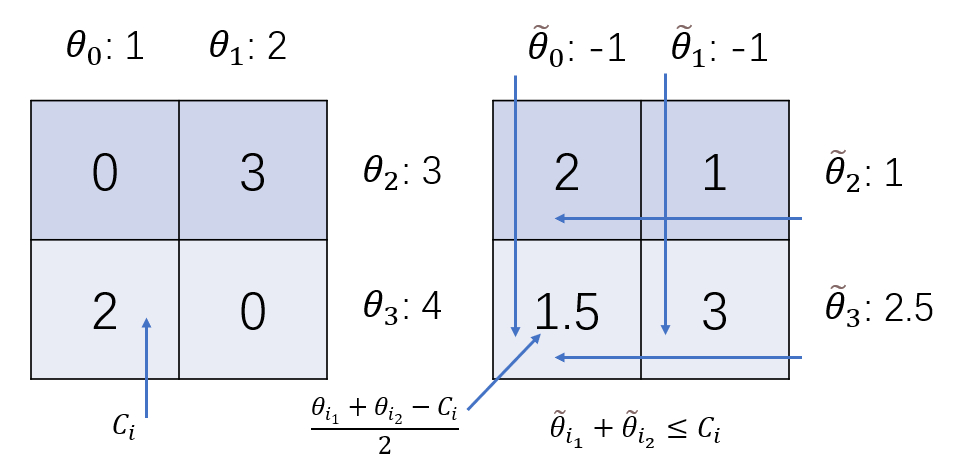
\includegraphics[width = \linewidth]{pic/shifting}
	\caption{Shifting on a 2$\times$2 matrix}
	\end{center}	
	\end{figure}


As we have got the $\tilde{\theta}$ in the $R^{D}$ and we also have another constraint area $\mathcal{R}^{C}$, we are sure that the $\hat{\vt} \in \mathcal{R}^{C}\cap\mathcal{R}^{D}$. However, The intersection of a sphere and a polytope can not be computed in $O(knm)$, where $k$ is a constant. We design a relaxation method. which divides the constraints into two parts, then we maximize the intersection of two hyperplanes and a hyper-ball. 

	\begin{figure}[h]
	\begin{center}	
	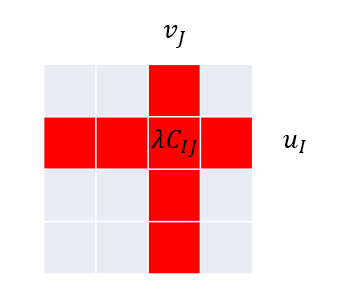
\includegraphics[width = \linewidth]{pic/divide}
	\caption{Selection of group $A_{IJ}$(red) and $B_{IJ}$(grey)}
	\end{center}	
	\end{figure}

\begin{thm}\label{area}(Two plane Screening for UOT) For every single primal variable $t_p$, let $A_p = \{ i \| 0\leq i<nm, i\mid m = I \vee i\mod m = J\}$, $B_p = \{ i \| 0\leq i<nm, i \notin A_p\}$. we can construct the specific area $\mathcal{R}^{S}_{IJ}$ for it.
 \begin{equation}
\begin{split} 
\mathcal{R}^S_{IJ} = \{\theta \|
\begin{aligned}
 &\sum_{l\in A_p}(\theta^{\tranT}\x_{l}\vt_l - \lambda \vc_l \vt)\leq 0 \\
 &\sum_{l\in B_p}(\theta^{\tranT}\x_{l}\vt_l - \lambda \vc_l \vt)\leq 0 \\
  &(\theta-\tilde{\theta})^{\tranT}(\theta-\y)\leq 0
\end{aligned}
\}
\end{split}
\label{eq:divide}
\end{equation}
\end{thm}
We divide the constraints into two groups $A_p$ and $B_p$ for every single $p$, this problem can be solved easily by the Lagrangian method in constant time, the computational process is in Appendix. A


\subsection{Screening Algorithms}

 \begin{algorithm}
 \caption{UOT Dynamic Screening Algorithm}
 \begin{algorithmic}[h]
 \renewcommand{\algorithmicrequire}{\textbf{Input:}}
 \renewcommand{\algorithmicensure}{\textbf{Output:}}
 \REQUIRE $\vt_0, S \in R^{n\times m}, S_{ij}=1, (i,j) = mi+j$
 \ENSURE $S$
 \STATE \text{Choose a solver for the problem.}
 \FOR {$k = 0 \text{ to } K$}
 \STATE $\text{Projection } \tilde{\theta} = \operatorname{Proj}(t^k)$ 
 \FOR {$i = 0 \text{ to } m$}
  \FOR {$j = 0 \text{ to } n$}
  \STATE $\mathcal{R}^{S} \Leftarrow \mathcal{R_{ij}}^S{(\tilde{\theta},t^k)}$
   \STATE $S \Leftarrow {S_{ij} = 0 \text{ if } \max_{\theta \in \mathcal{R}^S} {x_{(i,j)}}^{\tranT}\theta <\lambda c_{(i,j)} }$
 \ENDFOR
  \ENDFOR
 \FOR {$(i,j) \in \{(i,j)\|S_{ij}=0\}$}
  \STATE $\vt^k_{(i,j)} \Leftarrow 0$
  \ENDFOR
  \STATE $\vt^{k+1} = \operatorname{update}(\vt^k)$
 \ENDFOR
  
 \RETURN $\vt^{K+1}, S $ 
 \end{algorithmic} 
 \end{algorithm}

The screening method is irrelevant to the optimization solver you choose. We give the specific algorithm for $L_2$ UOT problem to show the whole optimization process. The $\operatorname{update}$ indicates the updating process for $\vt$ according to the optimizer you choose.\\












































\section{Experiments}
In this section, we show the efficacy of the proposed methods using a toy Gaussian model and the MNIST dataset.
\subsection{Screening Ratio}
\section{Conclusion}
Our algorithm is great, we are going to apply the method onto Sinkhorn
\bibliography{ref}
\bibliographystyle{plainnat}

%%%%%%%%%%%%%%%%%%%%%%%%%%%%%%%%%%%
%%%%%% SUPPLEMENT (OPTIONAL) %%%%%%
%%%%%%%%%%%%%%%%%%%%%%%%%%%%%%%%%%%

\clearpage
\appendix

\thispagestyle{empty}


% For one-column format, uncomment the following:
\onecolumn \makesupplementtitle
% For two-column format, uncomment the following:
%\twocolumn[ \makesupplementtitle ]

\section{FORMATTING INSTRUCTIONS FOR THE SUPPLEMENTARY MATERIAL}

Your supplementary material should go here. It may be in one-column or two-column format. To display the supplementary material in two-column format, comment out the line
\begin{verbatim}
\onecolumn \makesupplementtitle
\end{verbatim}
and uncomment the following line:
\begin{verbatim}
\twocolumn[ \makesupplementtitle ]
\end{verbatim}

Please submit your paper (including the supplementary material) as a single PDF file. Besides the PDF file, you may submit a single file of additional non-textual supplementary material, which should be a ZIP file containing, e.g., code.

If you require to upload any video as part of the supplementary material of your camera-ready submission, do not submit it in the ZIP file. Instead, please send us via email the URL containing the video location.

Note that reviewers are under no obligation to examine your supplementary material.

\section{MISSING PROOFS}

The supplementary materials may contain detailed proofs of the results that are missing in the main paper.

\subsection{Proof of Lemma 3}

\textit{In this section, we present the detailed proof of Lemma 3 and then [ ... ]}

\section{ADDITIONAL EXPERIMENTS}

If you have additional experimental results, you may include them in the supplementary materials.

\subsection{The Effect of Regularization Parameter}

\textit{Our algorithm depends on the regularization parameter $\lambda$. Here we illustrate the effect of this parameter on the performance of our algorithm [ ... ]}


\end{document}

